\documentclass[class=NTHU_thesis, crop=false]{standalone}
\begin{document}

\chapter{Background Estimation Strategy}
\label{chap:estimation_strategy}
Some SM processes show the same signature of the DM model, becoming the background in the analysis. The main background processes of the analysis are $Z$($\nu\nu$) + jets, $W$($l\nu$) + jets and $t\bar{t}$, shown in \cref{fig:Bkg-Processes}. In the $Z$($\nu\nu$) + jets process, the undetectable neutrinos in the final state are regarded as the missing energy. Thus once the jets are tagged as $b$-jets, the case will be background. In the $W$($l\nu$) + jets and $t\bar{t}$ processes, once the lepton is misidentified as the missing energy, the procedure will be interference as well.

\begin{figure}[!hbt]
	\captionsetup[subfigure]{labelformat=empty}
	\centering
	\subcaptionbox
	{$Z$($\nu\nu$) + jets
		\label{fig:Bkg-Processes-fig1}}
		{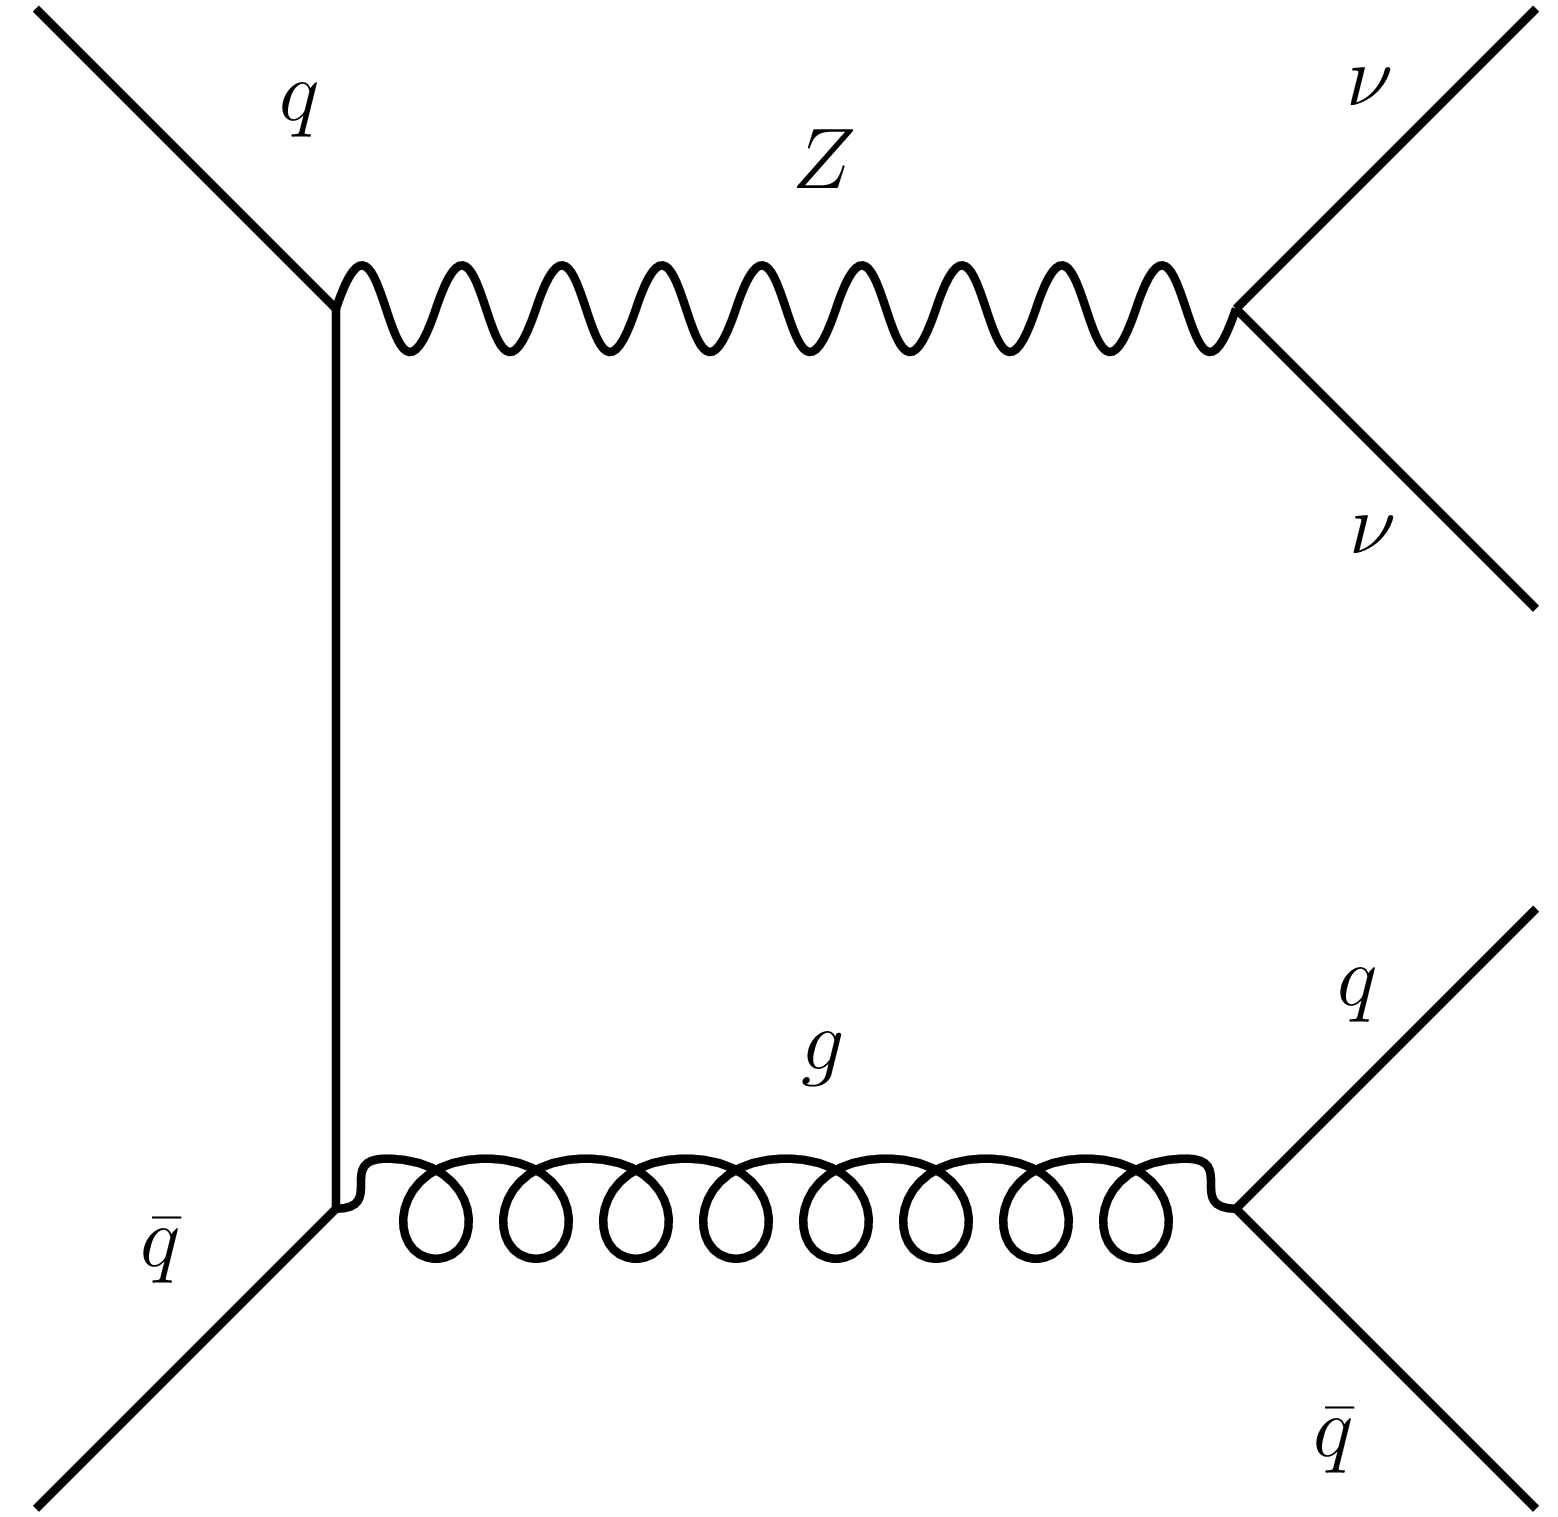
\includegraphics[width=0.32\linewidth]{Zvv.png}}
	\subcaptionbox
	{$W$($l\nu$) + jets
		\label{fig:Bkg-Processes-fig2}}
		{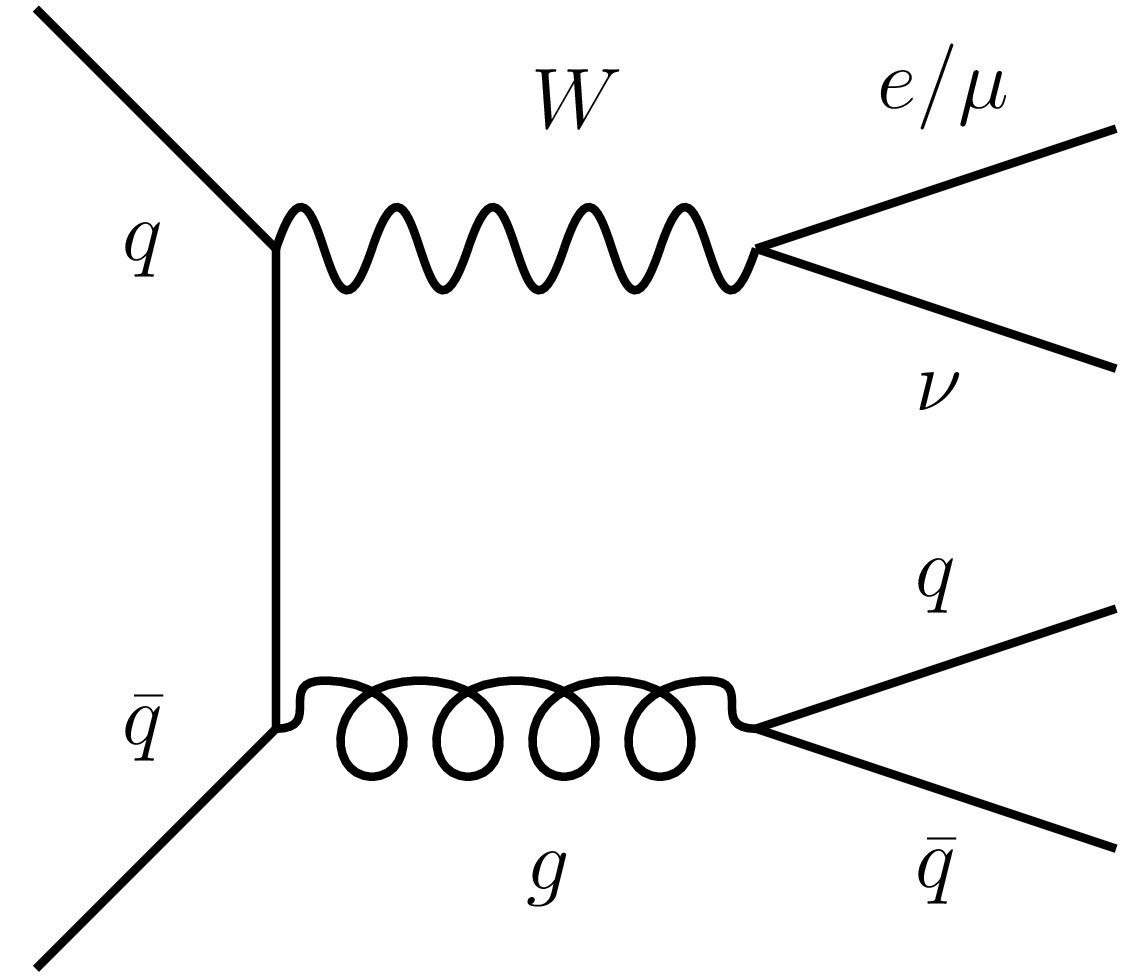
\includegraphics[width=0.32\linewidth]{Wlv.png}}
	\subcaptionbox
	{$t\bar{t}$
		\label{fig:Bkg-Processes-fig3}}
		{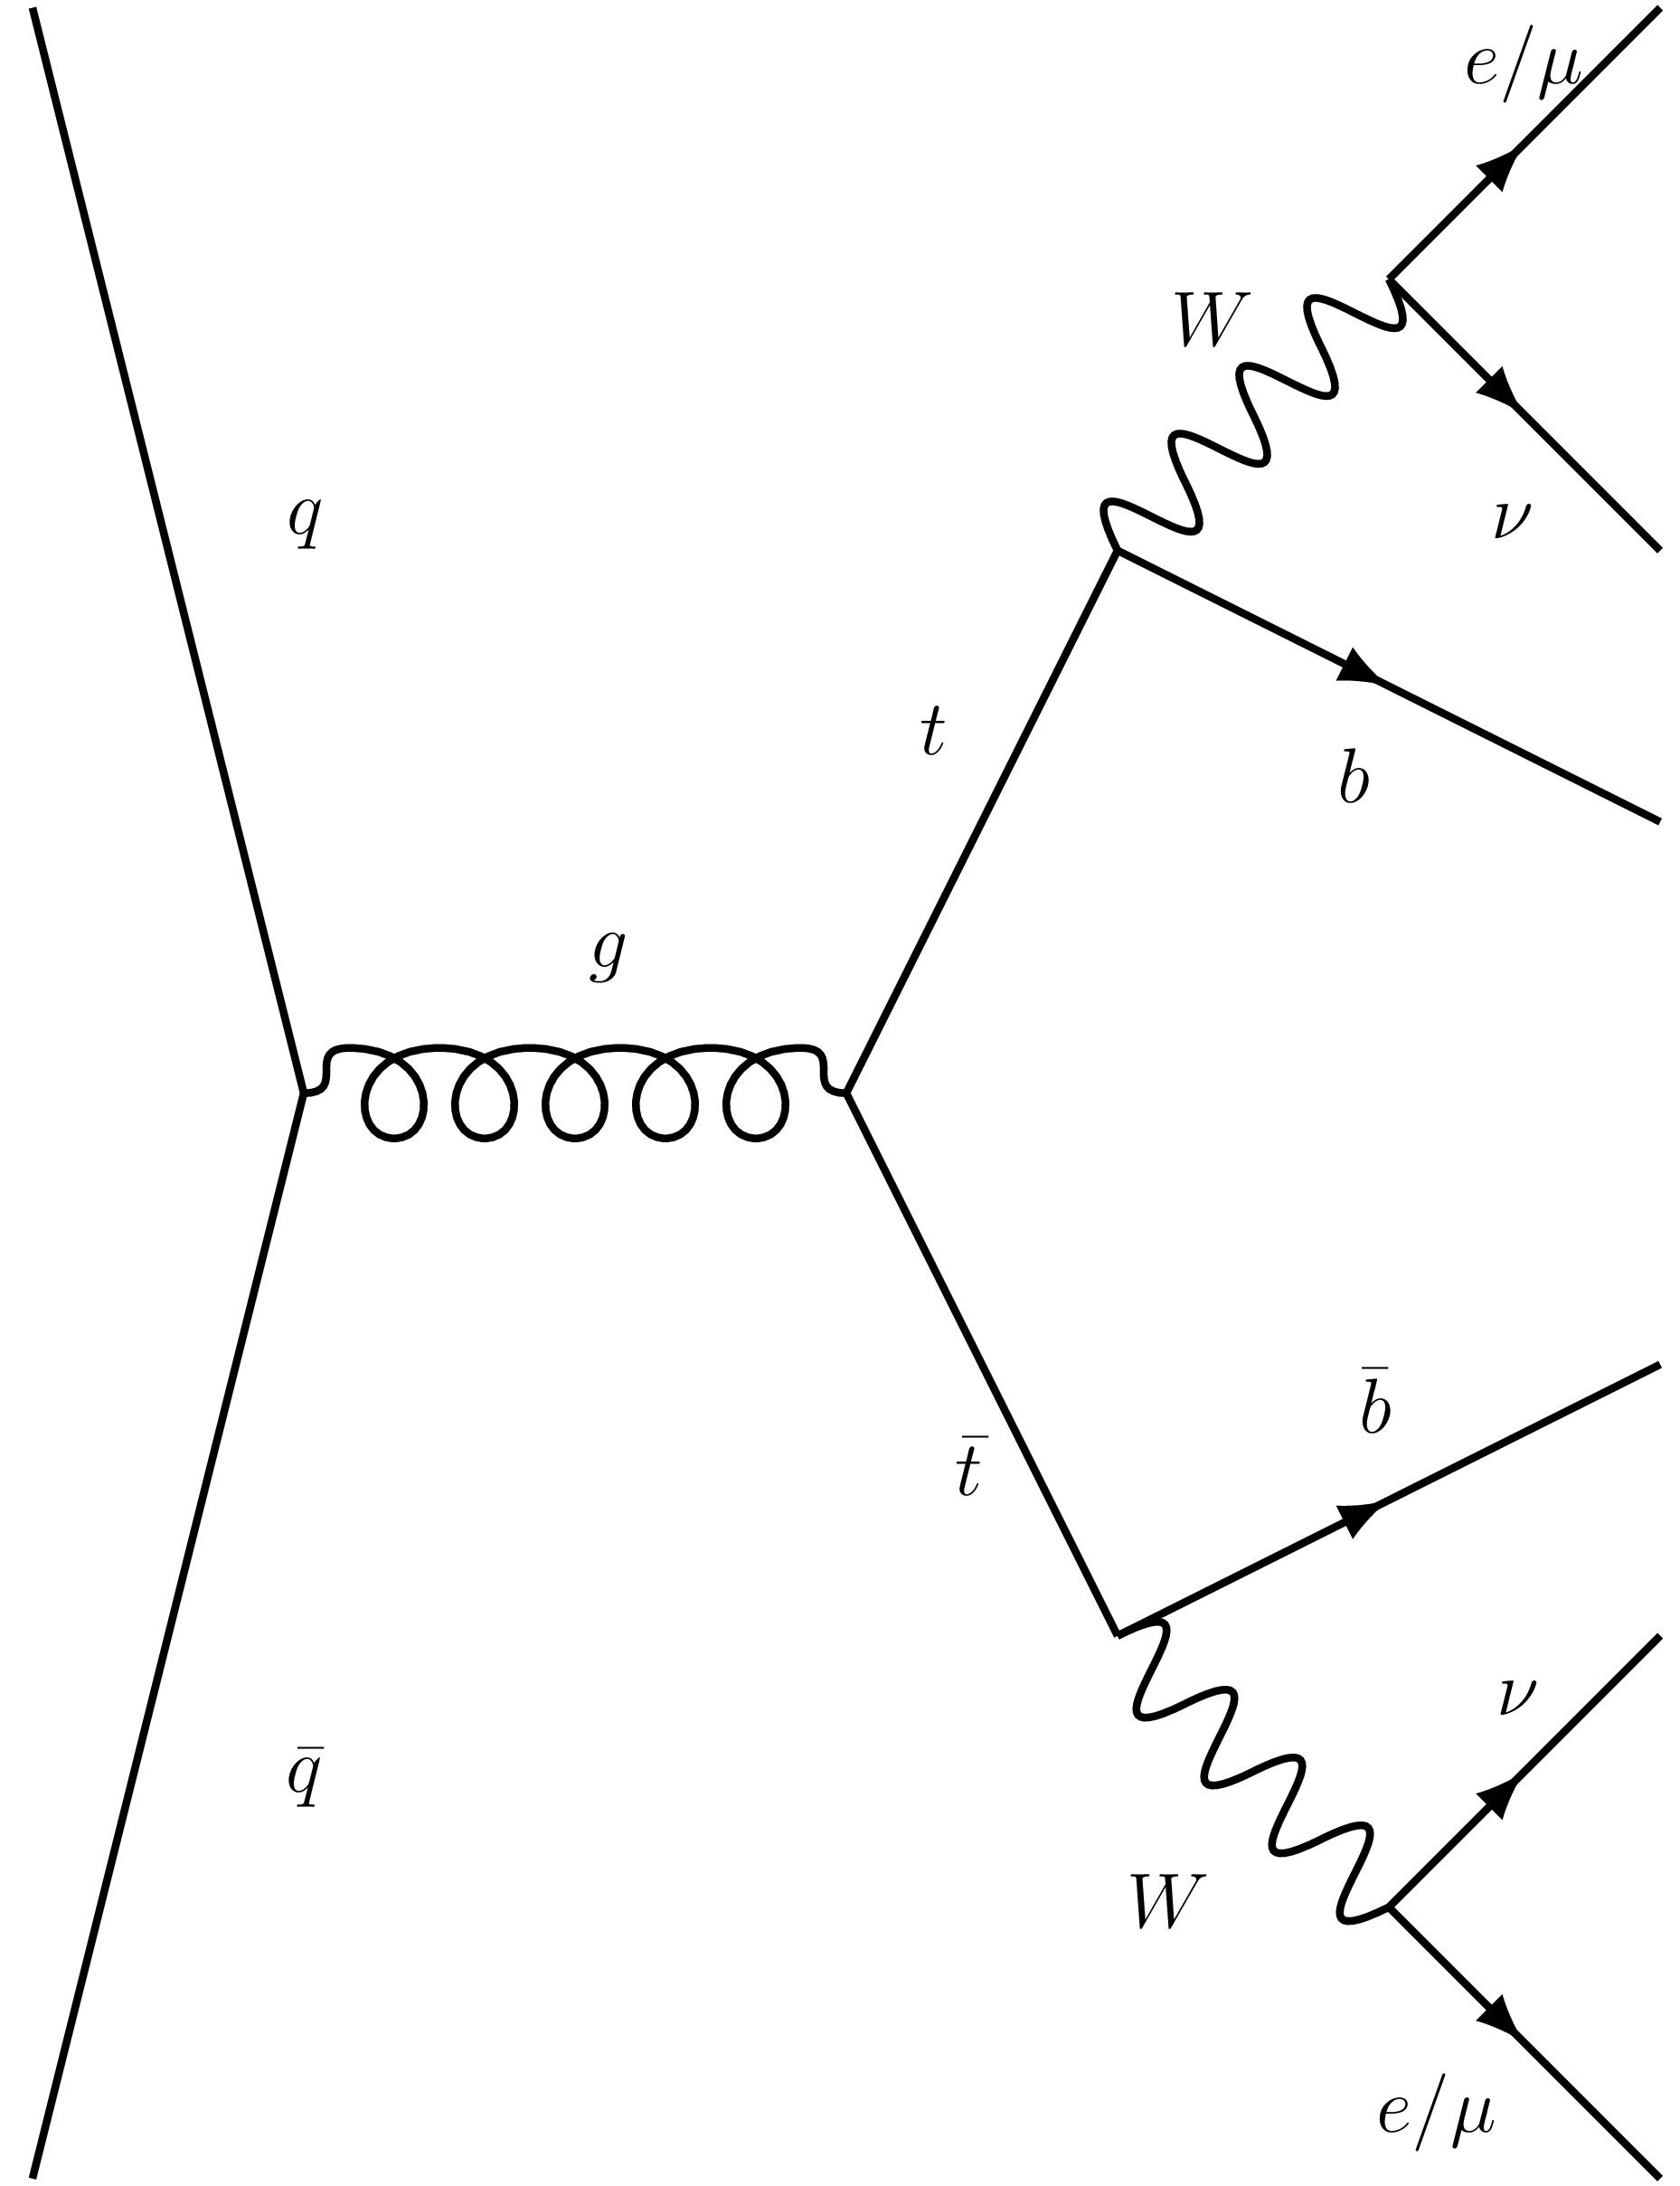
\includegraphics[width=0.32\linewidth]{ttbar.png}}
	\caption{The main background processes of the monoH analysis.}
	\label{fig:Bkg-Processes}
\end{figure}

To constrain the backgrounds, the control region (CR) strategy is used. Before defining the CR, the signal region (SR) is defined as where the signals are expected to show. The SR is required to have no lepton based on the model. Then the CR is defined as the orthogonal region to the SR. There are two CRs in this analysis, the one-muon CR and the two-lepton CR. The one-muon CR contains two processes, $W$($\mu\nu$) + jets and $t\bar{t}$, constraining $W$($l\nu$) + jets and $t\bar{t}$ in the SR. It requires different number of misidentified leptons, one in the SR but none in the one-muon CR. The two-lepton CR exploits the $Z$($ll$) + jets, constraining the $Z$($\nu\nu$) + jets process. Because it is not easy to simulate the misidentification as well as the kinematics of invisible neutrinos, these two CRs can constrain the background processes well.

\end{document}